\section{Auswertung}
\label{sec:Auswertung}
Jegliche Fehlerrechnung wurde mit der python-Bibliothek uncertainties \cite{uncertainties} absolviert.
Trotz dessen sind die Formeln für die Unsicherheiten in den jeweiligen Abschnitten angegeben.
Allgemeine Rechnungen wurden mit der python-Bibliothek numpy \cite{numpy} automatisiert. 
Die graphischen Untersützungen wurden mit Hilfe der python-Bibliothek matplotlib \cite{matplotlib} erstellt.
\subsection{Bestimmung der Untergrundrate}
Zu der Messung der Untergrundrate wurde ein Zeitintervall von $\symup{\Delta} t = \SI{300}{\second}$ gewählt.
Ingesamt ergaben sieben Messungen die Werte:
\begin{equation*}
    N_U = \{ 129, 143, 144, 136, 139, 126, 158 \}
\end{equation*}
Der Mittelwert der Untergrundrate beträgt
\begin{equation*}
    \bar{U}_N = 139.2857
\end{equation*}
\subsection{Bestimmung der Halbwertszeit von Vanadium}
\label{sub:Vana}
Bevor die Messdaten ausgewertet werden können, muss der Mittelwert der Hintergrundrate mit dem Zeitintervall von $\symup{\Delta} t = \SI{30}{\second}$
abgezogen werden. Dieser beträgt
\begin{equation*}
    \bar{U}_\text{N, \SI{30}{\second}} = 13.9286 \approx 14 \; \text{.}
\end{equation*}
Die Dezimalstellen des Mittelwerts wurden durch Runden eleminiert, da es nur ganze Vanadium-Kerne geben kann.\footnote{Es wurde nur bei der Tabelle gerundet, damit diese
übersichtlicher ist.}
In der Tabelle \ref{tab:vana} sind die instabilen Vanadium-Kerne ohne Abzug der Untergrundrate $\tilde{N}$ und die instabilen Vanadium-Kerne mit Abzug 
der Untergrundrate aufgetragen.
\begin{table}
    \centering
    \caption{Instabile Vanadium-Kerne}
    \label{tab:vana}
    \begin{tabular}{S[table-format=3.0] S[table-format=3.0] S[table-format = 3.0] @{${}\pm{}$} S[table-format = 2.2]
                    S[table-format=4.0] S[table-format=2.0] S[table-format = 2.0] @{${}\pm{}$} S[table-format = 1.2]}
        \toprule
        {$t \mathbin{/} \si{\second}$} & {$\tilde{N}$} & \multicolumn{2}{c} {$N$} & {$t \mathbin{/} \si{\second}$} & {$\tilde{N}$} & \multicolumn{2}{c} {$N$} \\
        \midrule
        30	&    189    & 175 & 13.23 & 690  &  35  & 21 & 4.59    \\
        60	&    197    & 183 & 13.53 & 720  &  19  & 5  & 2.25    \\
        90	&    150    & 136 & 11.66 & 750  &  28  & 14 & 3.75    \\
        120	&    159    & 145 & 12.04 & 780  &  27  & 13 & 3.62    \\
        150	&    155    & 141 & 11.88 & 810  &  36  & 22 & 4.70    \\
        180	&    132    & 118 & 10.87 & 840  &  25  & 11 & 3.33    \\
        210 &	 117    & 103 & 10.15 & 870  &  29  & 15 & 3.88    \\
        240 &	 107    & 93  &  9.65 & 900  &  18  & 4  & 2.02    \\
        270 &	 94     & 80  &  8.95 & 930  &  17  & 3  & 1.75    \\
        300 &	 100    & 86  &  9.28 & 960  &  24  & 10 & 3.17    \\
        330 &	 79     & 65  &  8.07 & 990  &  21  & 7  & 2.66    \\
        360 &	  69    & 55  &  7.42 & 1020 &  25  & 11 & 3.33    \\
        390 &	  81    & 67  &  8.19 & 1050 &  21  & 7  & 2.66    \\
        420 &	  46    & 32  &  5.66 & 1080 &  24  & 10 & 3.17    \\
        450 &	  49    & 35  &  5.92 & 1110 &  25  & 11 & 3.33    \\
        480 &	  61    & 47  &  6.86 & 1140 &  17  & 3  & 1.75    \\
        510 &	  56    & 42  &  6.49 & 1170 &  20  & 6  & 2.46    \\
        540 &	  40    & 26  &  5.11 & 1200 &  19  & 5  & 2.25    \\
        570 &	  45    & 31  &  5.57 & 1230 &  20  & 6  & 2.46    \\
        600 &	  32    & 18  &  4.25 & 1260 &  18  & 4  & 2.02    \\
        630 &	  27    & 13  &  3.62 & 1290 &  16  & 2  & 1.44    \\
        660 &	  43    & 29  &  5.39 & 1320 &  17  & 3  & 1.75    \\
    \bottomrule     
    \end{tabular}
\end{table}
Zu der Bestimmung der Halbwertszeit wird das Zerfallsgesetz $REFERENZ$ logarithmiert, so dass sich die Umformung
\begin{equation}
\ln \left (\frac{N}{N_0} \right ) = - \lambda t 
\end{equation}
Somit lässt sich eine lineare Ausgleichrechung mit der Geradengleichung
\begin{equation}
    y = at + b 
\end{equation}
durchführen. 
Für Regressionsparameter $a$ n und $b$ ergibt sich
\begin{align*}
    a &= \SI{-0.0032(2)}{\per\second} = - \lambda\\
    b &= \num{0.0213(1275)}
\end{align*}
\begin{figure}
    \centering
    \caption{Zerfallskurve von Vanadium}
    \label{fig:vana}
    \includegraphics{build/vana.pdf}
\end{figure}
Mit Hilfe der Gleichung $REFERENZ$ lässt sich die Halbwertszeit zu
\begin{equation*}
\tau = \SI{219(11)}{\second}
\end{equation*}
bestimmen.
Der Fehler der übrigen Kerne lässt sich mittels
\begin{equation}
    \symup{\Delta} N = \sqrt{N} 
\end{equation}
errechnen.
Nach der Gaußschen Fehlerfortpflanzung wird die Unsicherheit der Halbwertszeit durch
\begin{equation}
    \symup{\Delta} \tau = \frac{\ln \left (2 \right )}{\lambda^2} \symup{\Delta} \lambda
\end{equation}
\subsection{Bestimmung der Halbwertszeit von Rhodium}
Wie bereits in Abschnitt \ref{sub:Vana} muss der Mittelwert der Hintergrundrate abgezogen werden.
Da die übrigen Rhodium-Kerne mit einem Intervall von $\symup{\Delta} t = \SI{15}{\second}$ gemessen wurden, muss der Mittelwert der Untergrundrate
auf dieses Zeitintervall herunterskaliert werden.
\begin{equation*}
    \bar{U}_\text{N, \SI{15}{\second}} = 6.9644 \approx 7 \; \text{.}
\end{equation*}
Erneut wurden die  Dezimalstellen des Mittelwert Runden eleminiert (selbige Begründung).
In der Tabelle \ref{tab:vana} sind die instabilen Rhodium-Kerne ohne Abzug der Untergrundrate $\tilde{N}$ und die instabilen Rhodium-Kerne mit Abzug 
der Untergrundrate aufgetragen.
\begin{table}
    \centering
    \caption{Instabile Rhodium-Kerne}
    \label{tab:rho}
    \begin{tabular}{S[table-format=3.0] S[table-format=3.0] S[table-format = 3.0] @{${}\pm{}$} S[table-format = 2.2]
                    S[table-format=3.0] S[table-format=2.0] S[table-format = 2.0] @{${}\pm{}$} S[table-format = 1.2]}
        \toprule
        {$t \mathbin{/} \si{\second}$} & {$\tilde{N}$} & \multicolumn{2}{c} {$N$} & {$t \mathbin{/} \si{\second}$} & {$\tilde{N}$} & \multicolumn{2}{c} {$N$} \\
        \midrule
        15  &  667 & 660 & 25.69 & 345 & 36 & 29 & 5.39 \\
        30  &  585 & 578 & 24.04 & 360 & 38 & 31 & 5.57 \\
        45  &  474 & 467 & 21.61 & 375 & 34 & 27 & 5.20 \\
        60  &  399 & 392 & 19.80 & 390 & 40 & 33 & 5.74 \\
        75  &  304 & 297 & 17.23 & 405 & 21 & 14 & 3.74 \\
        90  &  253 & 246 & 15.68 & 420 & 35 & 28 & 5.29 \\
        105 &  213 & 206 & 14.35 & 435 & 33 & 26 & 5.10 \\
        120 &  173 & 166 & 12.88 & 450 & 36 & 29 & 5.39 \\
        135 &  152 & 145 & 12.04 & 465 & 20 & 13 & 3.61 \\
        150 &  126 & 119 & 10.91 & 480 & 24 & 17 & 4.12 \\
        165 &  111 & 104 & 10.20 & 495 & 30 & 23 & 4.80 \\
        180 &   92 & 85  & 9.22  & 510 & 30 & 23 & 4.80 \\
        195 &   79 & 72  & 8.49  & 525 & 26 & 19 & 4.36 \\
        210 &   74 & 67  & 8.19  & 540 & 28 & 21 & 4.58 \\
        225 &   60 & 53  & 7.28  & 555 & 23 & 16 & 4.00 \\
        240 &   52 & 45  & 6.71  & 570 & 20 & 13 & 3.61 \\
        255 &   56 & 49  & 7.00  & 585 & 28 & 21 & 4.58 \\
        270 &   53 & 46  & 6.78  & 600 & 17 & 10 & 3.16 \\
        285 &   41 & 34  & 5.83  & 615 & 26 & 19 & 4.36 \\
        300 &   36 & 29  & 5.39  & 630 & 19 & 12 & 3.46 \\
        315 &   37 & 30  & 5.48  & 645 & 13 & 6  & 2.45 \\
        330 &   32 & 25  & 5.00  & 660 & 17 & 10 & 3.16 \\
        \bottomrule     
    \end{tabular}
\end{table}
\begin{figure}
    \centering
    \caption{Zerfallskurve von Rhodium}
    \label{fig:rho}
    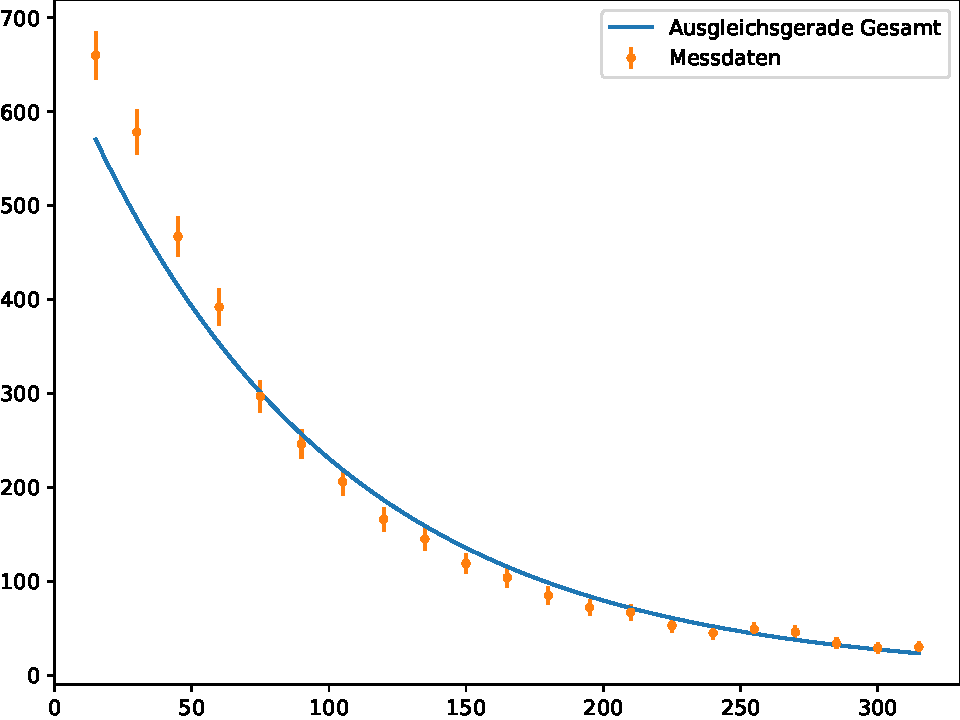
\includegraphics{build/rho.pdf}
\end{figure}
In der Abbildung \ref{fig:rho} ist die Zerfallskurve und dessen Ausgleichsgeraden aufgetragen. 
Einerseits ist die Ausgleichsgerade für beide Zerfallskanäle. 
Anderseits sind Ausgleichsgeraden für die einzelnen Zerfallskanäle aufgetragen.
Um die einzelnen Geraden zu ermitteln, ist es von Nöten den Zeitpunkt zu bestimmen, ab wann der langlebige Zerfallsprozess einsetzt.
Dieser kann der Abbildung \ref{fig:rho} grapisch entnehmen.
Dort ist zu erkennen, dass der langlebige Prozess ab $_lang = \SI{315}{\second}$ einsetzt.
Für die Gerade aller Messdaten 
\begin{equation}
    y_g = a_g t_g + b_g
\end{equation}
ergeben sich die Parameter zu 
\begin{align*}
    a &= \SI{-0.0057}{\second} \\
    b &= \SI{}{}
\end{align*}
Die Parameter der Ausgleichgerade ab $t_lang$
\begin{equation}
    y_l = c t_l + b_l
\end{equation}
\begin{figure}
    \centering
    \caption{Zerfallskurve von Rhodium}
    \label{fig:rhoall}
    \includegraphics{build/rhoall.pdf}
\end{figure}